\chapter{What is \texttt{pychoacoustics}?}

\texttt{pychoacoustics} is a software for programming and running experiments in auditory psychophysics (psychoacoustics). The software contains a set of predefined experiments that can be immediately run after installation. Importantly \texttt{pychoacoustics} is designed to be extensible so that users can add new custom experiments with relative ease. Custom experiments are written in Python, a programming language renowned for its clarity and ease of use. The application is divided in two graphical windows a) the ``response box'', shown in Figure~\ref{fig:response_box}, with which listeners interact during the experiment b) the control window, shown in Figure~\ref{fig:control_window}, that contains a series of widgets (choosers, text field and buttons) that are used by the experimenter to set all of the relevant experimental parameters, which can also be stored and later reloaded into the application. %Writing experiments for \texttt{pychoacoustics} gives immediate access to an extensive set of facilities for the selection, storage and retrieval of experimental parameters, stimulus presentation, randomization of experimental blocks, as well as storage and processing of experimental responses.

\begin{figure}[!h]
   \caption{The Response Box}
   \centering
   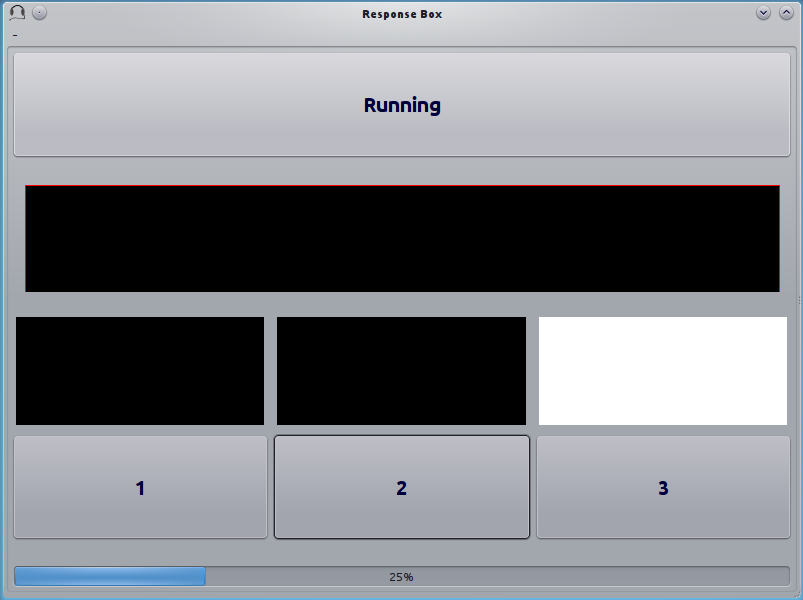
\includegraphics[scale=0.6]{Figures/response_box.png}
   \label{fig:response_box}
 \end{figure}

\begin{figure}[!h]
   \caption{The Control Window}
   \centering
   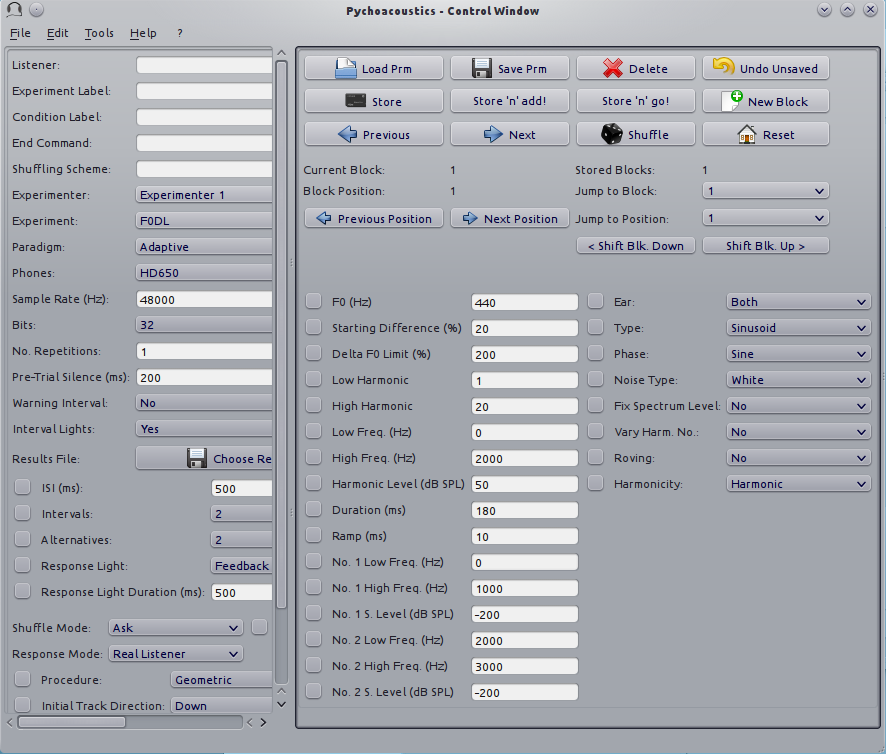
\includegraphics[scale=0.55]{Figures/control_window.png}
   \label{fig:control_window}
 \end{figure}

I started writing \texttt{pychoacoustics} for fun and for the sake of learning around 2008 while doing my PhD with Professor Chris Plack at Lancaster University. At that time we were using in the lab a MATLAB program called the ``Earlab'' written by Professor Plack. \texttt{pychoacoustics} has been greatly influenced and inspired by the ``Earlab'', and it reproposes many of the same features that the ``Earlab'' provides. For this reason, as well as for the patience he had to teach me audio programming I am greatly indebted to Professor Plack. %The ``Earlab'' has a venerable history, and was ported to various platforms and programming languages before reaching its MATLAB incarnation. \texttt{pychoacoustics} was initially written using the wxWidgets toolkit, and was 



%%% Local Variables: 
%%% mode: latex
%%% TeX-master: "pychoacoustics_manual"
%%% End: 

